% Sign structure of the fermionic toric code, and why the NQS stack feels it.
% Companion to notes/fermionic_plateau_diagnosis.md and notes/handoff_fermionic_tc.md.
% Compile: pdflatex fermionic_sign_problem.tex  (twice, for refs)
\documentclass[11pt]{article}
\usepackage[margin=1.1in]{geometry}
\usepackage{amsmath,amssymb,amsthm}
\usepackage{booktabs}
\usepackage{tikz}
\usepackage[colorlinks=true,linkcolor=blue!60!black,citecolor=blue!60!black,urlcolor=blue!60!black]{hyperref}
\usepackage{microtype}

\newcommand{\Av}{A_v}
\newcommand{\Bp}{B_p}
\newcommand{\Bt}{\tilde B_p}
\newcommand{\ket}[1]{|#1\rangle}
\newcommand{\bra}[1]{\langle#1|}
\newcommand{\braket}[2]{\langle#1|#2\rangle}
\newcommand{\sx}{\sigma^x}
\newcommand{\sy}{\sigma^y}
\newcommand{\sz}{\sigma^z}

\title{The sign problem of the 3D fermionic toric code:\\
background, mechanism, and consequences for NQS}
\author{toric-code-nqs project notes}
\date{August 7, 2026}

\begin{document}
\maketitle

\begin{abstract}
\noindent
The bosonic 3D toric code (bTC) in fields $h_x,h_z$ is sign-problem-free and our
real-weight NQS stack handles it; the same code with $h_y\neq0$ is sign-full but
trainable with complex weights. The fermionic toric code (fTC) is sign-full
\emph{already at zero field}, and our benchmark runs (2026-08-06) show the
production ansatz converging not to the ground state but to a well-defined
impostor: the optimal wavefunction confined to the positive-sign half of the
ground-state support, at $\delta\approx30\%$ energy error. This note collects
the background needed to understand all of this in one place: a 2D warm-up
(where the standard fermionic dressing is a full star and the zero-field ground
state remains positive---isolating exactly what 3D adds), what a sign
problem is (and how the QMC and VMC versions differ), why the bTC is safe, where
the fTC sign structure comes from microscopically, what is exactly known about
it at $h=0$, why the variational optimizer---not the ansatz---is the failing
component, whether the problem is ``intrinsic,'' and what the literature offers.
\end{abstract}

\tableofcontents

%=====================================================================
\section{The two models}

Qubits live on the edges of an $L^3$ cubic lattice (PBC). The bosonic toric
code in uniform fields is
\begin{equation}
H_{\mathrm{bTC}} \;=\; -J\sum_v \Av \;-\; J\sum_p \Bp
\;-\; h_x\sum_i \sx_i \;-\; h_y\sum_i \sy_i \;-\; h_z\sum_i \sz_i ,
\qquad
\Av=\!\!\prod_{e\in\mathrm{star}(v)}\!\!\sx_e,\quad
\Bp=\!\!\prod_{e\in\partial p}\!\!\sz_e ,
\end{equation}
with $6$-edge stars and $4$-edge plaquette boundaries. The fermionic toric code
keeps the stars and \emph{decorates} each plaquette with two $\sx$ on the
body-diagonal corner edges $d_p=\{e_+,e_-\}$ at
$\mathrm{ctr}(p)\pm\tfrac12(\hat e_a+\hat e_b+\hat e_c)$
(this is the minimal $2$-edge alternative, implemented in
\texttt{tc3d/fermionic\_decoration.py}, to the $10$-edge dressing of
Ref.~\cite{WangLevin2014}):
\begin{equation}
H_{\mathrm{fTC}} \;=\; -J\sum_v \Av \;-\; J\sum_p \Bt \;-\; h_x\sum_i \sx_i
\;-\; h_z\sum_i \sz_i,
\qquad
\Bt \;=\; \Big(\prod_{e\in\partial p}\sz_e\Big)\,\sx_{e_+}\sx_{e_-} .
\end{equation}
All $\Av,\Bt$ mutually commute (verified to $0$ violations at $L=2,3$;
translation invariance extends this to all $L$), the $\sz$- and $\sx$-supports
of each $\Bt$ are disjoint, and at $h=0$ the model is frustration-free with
$E_0=-4L^3$ exactly, same as the bTC. The physics that differs is the
\emph{statistics of the point excitation}: a $\sz$ string must be dressed with
$\sx$ to commute with the $\Bt$'s, a closed dressed loop is a conserved Wilson
loop, but an \emph{open} dressed string necessarily leaves one violated
plaquette at each endpoint---each end carries charge (violated star)
\emph{and} flux (violated plaquette). That charge--flux composite is a fermion;
the impossibility of a flux-free open string is the operational statement of
its statistics, in the spirit of the string picture of emergent fermions of
Levin and Wen~\cite{LevinWen2003}. The same structure---$\Bp$ dressed by
$\sx$ pairs, i.e.\ a $\mathbb{Z}_2$ gauge theory whose Gauss law/flux terms are
modified so the charge is fermionic---is precisely what exact lattice
bosonization produces in 2D~\cite{ChenKapustinRadicevic2018} and
3D~\cite{ChenKapustin2019}.

%=====================================================================
\section{Warm-up: the fermionic toric code in 2D}
\label{sec:2d}

The 2D construction is the right place to build intuition, because it is easy
to draw \emph{and} because it turns out to behave completely differently at
zero field. The standard 2D fermionic plaquette dresses $\Bp$ with $\sx$ on
the four edges incident to one of its corners, say the southwest vertex
$v(p)$ (on the two shared edges $\sx$ and $\sz$ coincide, giving
$\sy$ up to phase):

\begin{center}
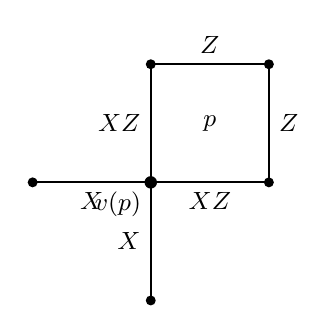
\begin{tikzpicture}[scale=1.5, every node/.style={font=\small}]
% plaquette edges
\draw[thick] (0,1) -- (1,1) node[midway,above] {$Z$};
\draw[thick] (1,0) -- (1,1) node[midway,right] {$Z$};
\draw[thick] (0,0) -- (0,1) node[midway,left] {$XZ$};
\draw[thick] (0,0) -- (1,0) node[midway,below] {$XZ$};
% external star edges
\draw[thick] (-1,0) -- (0,0) node[midway,below] {$X$};
\draw[thick] (0,-1) -- (0,0) node[midway,left] {$X$};
% vertices
\fill (0,0) circle (1.5pt) node[below left] {$v(p)$};
\fill (1,0) circle (1.2pt);
\fill (0,1) circle (1.2pt);
\fill (1,1) circle (1.2pt);
\fill (-1,0) circle (1.2pt);
\fill (0,-1) circle (1.2pt);
\node at (0.5,0.5) {$p$};
\end{tikzpicture}
\qquad\qquad
\raisebox{2.1em}{$\displaystyle \Bt^{\rm 2D} \;=\; A_{v(p)}\,\Bp$}
\end{center}

\noindent
The four $\sx$ form exactly the star of $v(p)$: the 2D dressing \emph{is a
stabilizer of the bosonic code}. That has an immediate structural consequence:
\begin{equation}
\big\langle A_v,\ \Bt^{\rm 2D}\big\rangle
\;=\;\big\langle A_v,\ A_{v(p)}\Bp\big\rangle
\;=\;\big\langle A_v,\ \Bp\big\rangle ,
\end{equation}
i.e.\ the stabilizer \emph{group} is unchanged. At $h=0$ the 2D fermionic and
bosonic toric codes therefore have the \emph{same} ground state---positive,
sign-free. What changes is only which excitations are ``elementary'': a lone
violation of $\Bt^{\rm 2D}$ is the composite $\epsilon=e\times m$, the fermion
that already existed in the bosonic spectrum. The 2D fTC is the toric code
with its fermion promoted to fundamental charge; the models differ in their
\emph{excitations} and hence in their response to fields (the perturbed
Hamiltonian is non-stoquastic as written, and the transition is driven by
condensing a fermion), but not in their zero-field ground state.

The ``evenness'' intuition makes this transparent in the amplitude-propagation
language. The rule $\Bt^{\rm 2D}\ket\psi=\ket\psi$ reads
$\psi(s\oplus\mathrm{star}_{v(p)})=\varepsilon_p(s)\psi(s)$ with
$\varepsilon_p(s)=(-1)^{|\partial p\cap s|}$---formally sign-carrying. But the
group still contains the \emph{diagonal} $\Bp$, whose $+1$ constraint confines
the ground-state support to even-parity configurations, $\varepsilon_p\equiv+1$
there; and star flips preserve every boundary parity (a star shares $0$ or $2$
edges with every $\partial p$, in 2D and 3D alike). The sign factor exists in
the algebra but is never \emph{activated} on the support.

\paragraph{What 3D changes.}
In 2D, binding flux to charge is a relabeling inside the same phase, because
both $e$ and $m$ are points. In 3D the flux is a \emph{loop}: no relabeling
binds it to a point charge, and a $\mathbb{Z}_2$ gauge theory whose point
charge is a fermion is a genuinely distinct phase
\cite{LevinWen2003,WangLevin2014,ChenKapustin2019}. Correspondingly, any
dressing built from whole stabilizers (e.g.\ $A_v\Bp$ in 3D) would again leave
the group---and the positive ground state---untouched, fermionizing nothing.
A faithful 3D fermionic TC \emph{must} change the stabilizer group. The
minimal such dressing is our body-diagonal $\sx$ pair: it is not a product of
stabilizers (the gap changes from $4$ to $8$), there is no longer any diagonal
plaquette operator confining the support to even parities, and---as
Sec.~\ref{sec:origin} shows---the pair overlaps neighboring boundaries an
\emph{odd} number of times, so the sign factor activates. The zero-field sign
structure of the 3D fTC is, in this precise sense, the cost of making the
fermion genuine rather than relabeled.

%=====================================================================
\section{What ``sign problem'' means, twice}
\label{sec:defs}

\subsection{QMC: stoquasticity and Perron--Frobenius}

Fix a product basis $\{\ket{s}\}$. A Hamiltonian is \emph{stoquastic} in that
basis if all off-diagonal matrix elements are $\le 0$
\cite{BravyiDiVincenzoOliveiraTerhal2008}. Then $e^{-\beta H}$ has nonnegative
entries, path-integral weights are probabilities, and QMC sampling is
sign-free; by Perron--Frobenius the ground state can be chosen with
$\psi(s)\ge 0$ for all $s$. Non-stoquasticity makes path weights of mixed sign;
observables become ratios of exponentially cancelling sums, with relative
errors growing like $e^{\beta N \Delta f}$. Generic sign problems are
NP-hard to cure \cite{TroyerWiese2005}; deciding/curing stoquasticity by local
basis changes is itself hard in general
\cite{MarvianLidarHen2019,KlassenTerhal2019}, though systematic easing is
sometimes possible \cite{Hangleiter2020}.

Two facts to keep straight:
(i) stoquasticity is a \emph{basis-dependent} property of $H$;
(ii) a positive ground state is a property of a \emph{state in a basis}. The
useful invariant question is whether \emph{any} local basis change makes the
problem sign-free (Sec.~\ref{sec:intrinsic}).

\subsection{VMC/NQS: the sign problem migrates into the optimizer}

Variational Monte Carlo has no path integral and no weight cancellation:
$E[\psi]=\mathbb{E}_{s\sim|\psi|^2}\,E_{\rm loc}(s)$ is estimated from
$|\psi(s)|^2\ge0$ regardless of signs. So VMC has no sign problem \emph{of the
QMC kind}. What it has instead:
\begin{itemize}
\item \textbf{Representation:} a log-amplitude ansatz
$\psi(s)=e^{\log\psi(s)}$ with \emph{real} $\log\psi$ outputs strictly
positive $\psi$---a sign-full ground state is outside its image entirely.
Complex parameters ($\log\psi=a+ib$, $\psi=e^a e^{ib}$) restore expressivity;
a negative amplitude is $b=\pi$.
\item \textbf{Optimization:} even when the target is representable, the
\emph{energy landscape over phases} can be rugged, with sign-structure local
minima and barriers \cite{SzaboCastelnovo2020,Bukov2021,Westerhout2020}. The
sampling measure compounds this: MCMC draws from $|\psi|^2$ of the
\emph{current} state, so regions where the current state has no weight are
never visited, and the only gradient signal about them enters through
off-diagonal terms of $E_{\rm loc}$.
\end{itemize}
Our results below are a textbook instance of the second bullet.

%=====================================================================
\section{Why the bosonic TC is safe}

\subsection{$h_y=0$: stoquastic, positive, real weights suffice}
In the computational $\sz$ basis, $\Bp$ and $h_z\sz$ are diagonal; the
off-diagonal operators are $-J\Av$ and $-h_x\sx$, both pure permutations with
coefficients $-J,-h_x\le0$ for $J,h_x\ge0$. Hence $H_{\mathrm{bTC}}(h_y{=}0)$
is stoquastic, the ground state is positive, real $\log\psi$ is fully
expressive, and both our NQS track and the QMC benchmark track (ParaToric)
live in this regime. This is why the entire tuning program (dual-basis
gridinv, FSS campaigns) never met a sign.

\subsection{$h_y\neq0$: sign-full but perturbatively connected}
$-h_y\sy$ has matrix elements $\mp i h_y$: mixed sign (indeed complex), so
stoquasticity is lost and the ground state acquires genuine phases. Yet our
complex-weight runs at $h_y=0.4$ trained without incident (validated
2026-07-21). The reason is \emph{continuity}: at $h_y=0$ the ground state is
positive; switching on $h_y$ deforms it smoothly, $\ket{\psi(h_y)}=
\ket{\psi_+}+O(h_y)$, with phases that grow from zero and amplitudes that
remain nonzero across the relevant configuration space. The phase-flat initial
network sits \emph{inside the basin} of the true state: every SR step gets
gradient signal from configurations it already samples, and no global phase
rearrangement is ever required. Sign-full $\neq$ hard; what matters is whether
the target is reachable by a descent path from the (inevitably phase-flat)
initialization.

%=====================================================================
\section{Origin of the fTC sign structure at $h=0$}
\label{sec:origin}

\subsection{Monomial matrices and the parity factor}
In the $\sz$ basis, $\Bt$ is not diagonal but is the next best thing, a
\emph{signed permutation} (monomial matrix): with $\varepsilon_p(s)=
(-1)^{|\partial p\,\cap\,s|}$ the boundary parity of the down-spins of $s$,
\begin{equation}
\Bt\ket{s}=\varepsilon_p(s)\,\ket{s\oplus d_p},
\qquad\text{so}\qquad
\bra{s\oplus d_p}(-J\Bt)\ket{s}=-J\,\varepsilon_p(s)=\mp J .
\label{eq:monomial}
\end{equation}
Positive off-diagonal elements occur (empirically a $\approx50/50$ split over
random $s$): the fTC is \emph{non-stoquastic in this basis at any field,
including zero}, and Perron--Frobenius positivity is lost.

\subsection{Why signs actually develop: the odd-overlap mechanism}
Stabilizer eigenvalue equations propagate amplitudes exactly. For the ground
state ($\Av\ket\psi=\Bt\ket\psi=+\ket\psi$),
\begin{equation}
\psi(s\oplus \mathrm{star}_v)=\psi(s),
\qquad
\psi(s\oplus d_p)=\varepsilon_p(s)\,\psi(s).
\label{eq:rules}
\end{equation}
A natural objection: starting from $\ket{0\cdots0}$ (even parity everywhere),
don't all flips preserve evenness, so that $\varepsilon\equiv+1$ along any
path? For \emph{star} flips, yes---a star shares $0$ or $2$ edges with every
plaquette boundary, so parities are preserved; this is exactly why the bTC
ground state is positive, and why the 2D fermionic code of
Sec.~\ref{sec:2d}---whose dressing is a full star---stays sign-free at $h=0$.
The 3D decoration pairs break the argument: a pair
$d_p$ (two normal-oriented edges at diagonally opposite corners of $p$,
displaced $\pm\tfrac12$ out of plane) shares exactly \emph{one} edge with the
boundaries of certain neighboring plaquettes ($192$ such odd overlaps at
$L=2$). Flipping $d_p$ therefore makes some other boundary parity odd, and the
\emph{next} plaquette action picks up $\varepsilon=-1$:
\begin{equation}
\ket{0\cdots0}
\;\xrightarrow{\;\Bt[p]\;}\;
\ket{d_p}\ (\text{some } \varepsilon_q \text{ now } -1)
\;\xrightarrow{\;\Bt[q]\;}\;
-\ket{d_p\oplus d_q}.
\end{equation}
Sign structure is an interference effect between stabilizers: the $\sx$ half of
one feeds the $\sz$ half of another. (Commutativity survives because oddness is
reciprocal, $|d_p\cap\partial q|$ odd $\Leftrightarrow$ $|d_q\cap\partial p|$
odd.)

\subsection{Exact solution at $h=0$: a signed stabilizer state}
Because $H(h{=}0)$ is a commuting stabilizer Hamiltonian, breadth-first
propagation of rules \eqref{eq:rules} from $\psi(0\cdots0)=+1$ constructs a
ground state exactly (no diagonalization; \texttt{tests/test\_fermionic.py}).
At $L=2$:
\begin{itemize}
\item The orbit (support) has $2^{15}=32{,}768$ states: over GF(2) the $8$ star
masks have rank $7$ and the $24$ pair masks add rank $8$.
\item The support splits $18{,}432$ positive / $14{,}336$ negative
($56.25\%/43.75\%$): the state is strongly sign-full.
\item The sign is an exact function of the $24$ \emph{flux tokens}
$t_p(s)=\varepsilon_p(s)$: the support collapses to $64$ token classes, each
carrying a single sign. Structural reason: sign-changing moves (pair flips
with odd overlap) always change tokens; token-preserving moves (stars) never
change signs. Consistent with the general theory of stabilizer states, the
sign is a GF(2) \emph{quadratic form} over these token bits.
\item By contrast, in the Hadamard-rotated (dual) basis the sign-carrying
moves change \emph{no} star token (faces overlap stars evenly): the entire
dual-frame support has one token vector while signs vary. No function of dual
star tokens can represent the state---the reason \texttt{--dual\_basis} is
fundamentally, not incidentally, bosonic-only.
\end{itemize}

%=====================================================================
\section{What the NQS actually does: the positive-sector trap}
\label{sec:trap}

Benchmark (2026-08-06, $L=2$ PBC, $h=0$, complex-weight
\texttt{ToricCNN\_gridinv}, exact $E_0=-32$):

\begin{center}
\begin{tabular}{lccccl}
\toprule
run & final $E$ & $\delta=\frac{|E-E_0|}{|E_0|}$ & Vscore & fate \\
\midrule
tune-rect winner (A) & $-22.5194$ & $29.6\%$ & $3\times10^{-4}$ & guard-killed, step 87\\
old workhorse (B) & $-22.5166$ & $29.6\%$ & $1\times10^{-3}$ & guard-killed, step 187\\
A, guard off, $+400$ iters & $-22.5211$ & $29.6\%$ & $3\times10^{-9}$ & never escaped\\
\bottomrule
\end{tabular}
\end{center}

Diagnosis (fresh samples from the trapped checkpoint, checked against the
exact solution; \texttt{notes/fermionic\_plateau\_diagnosis.md}): all $8192$
samples lie on the true support \emph{and} in its positive-sign half; the
network phases are flat to $10^{-4}$ rad; every plaquette shows
$\langle\Bt\rangle=0.605$ uniformly. The energy closes exactly:
within the positive half, star flips and the $\varepsilon=+1$ pair flips act
\emph{stoquastically} (contribute $-8$ and $-24\times0.605$), while
$\varepsilon=-1$ pair flips lead to the zero-weight negative half and
contribute nothing:
\begin{equation}
E_{\rm trap}=-8-24\times0.605=-22.52,
\qquad
0.605=\Pr\big[\varepsilon_p(s)=+1\,\big|\,s\in\text{positive half}\big].
\end{equation}
The trapped state is (essentially) the ground state of $H$ restricted to the
positive-sign sector---SR solved the sign-free restriction of the problem to
machine precision, which is why the plateau is an SR fixed point with
$\mathrm{Vscore}\sim10^{-9}$.

\paragraph{Why escape fails.}
Reaching the true ground state requires growing $\pi$-phased amplitude on
$44\%$ of the support \emph{coherently}: each plaquette term rewards relative
phase $0$ or $\pi$ in a specific correlated pattern; half-way phases
contribute nothing and wrong signs contribute with reversed sign. Every smooth
path from the phase-flat state to the target therefore first \emph{raises}
the energy (and dramatically raises the variance)---a first-order-like barrier
in wavefunction space. The observed ``divergence spikes'' were escape
attempts; with the guard disarmed they relax back on their own. Meanwhile the
sampling measure $|\psi|^2$ never visits the negative half, so the only
gradient signal about it enters through off-diagonal terms of $E_{\rm loc}$:
weak, noisy, and opposed by the barrier. This is the precise sense in which
\emph{the sign problem does not disappear in VMC---it migrates from the
sampler into the optimizer.}

\paragraph{Contrast with $h_y\neq0$ bTC.}
Same complex architecture, same optimizer---but there the target is
continuously connected to the positive state, phases grow from zero inside the
sampled region, and no sector is ever weightless. Here the target's sign
structure is $O(1)$, discrete, and macroscopically disconnected from the
initialization. Sign-fullness is not the obstacle; the \emph{topology of the
descent path} is.

%=====================================================================
\section{Is the fTC sign problem intrinsic?}
\label{sec:intrinsic}

Stoquasticity is basis-dependent, so one must ask whether some \emph{local}
transformation removes the sign. Three levels:
\begin{enumerate}
\item \textbf{At $h=0$, state level: not intrinsic.} The ground state is a
stabilizer state; a Clifford circuit maps it to a product state, and its sign
rule is exactly known (quadratic form over tokens). Nothing obstructs writing
it positively \emph{in some basis}---indeed this is the ``Clifford
disentangler'' idea in \texttt{notes/nqs\_architecture.md}: conjugate
$H_{\rm fTC}$ by a Clifford mapping $\{\Av,\Bt\}\to\{\Av,\Bp\}$. The catch is
what happens to the \emph{field terms}: single-site $\sx_i,\sz_i$ conjugate
into higher-weight Pauli strings, i.e.\ the perturbed model in the cured basis
is a different (still local, but not single-site-field) Hamiltonian. Whether
its NQS/QMC treatment is easier is an open engineering question, not a free
lunch.
\item \textbf{As a phase of matter: genuinely subtle.} In 3D, the
$\mathbb{Z}_2$ gauge theory with fermionic point charge is a distinct phase
from the bosonic one (the statistics of the point particle is a universal
invariant; cf.~\cite{LevinWen2003,ChenKapustin2019,WangLevin2014}), so no
finite-depth circuit maps fTC to bTC \emph{as Hamiltonian families}. The
modern ``intrinsic sign problem'' program
\cite{SmithGolanRingel2020,GolanSmithRingel2020} gives criteria (in 2D, via
chiral central charge and the spectrum of topological spins) for when a whole
phase admits \emph{no} stoquastic representative. Caution against
overclaiming in either direction: the plain 2D toric code contains a fermion
($\epsilon=e\times m$) and is nevertheless sign-free; and recent work shows
twisted quantum doubles---long suspected of intrinsic sign problems---admit
sign-problem-free representatives \cite{TwistedDoubles2025}. For our specific
3D fTC we should treat ``is there a local sign-curing basis at finite field''
as open.
\item \textbf{For NQS practice: the operative question is different.} We do
not need a stoquastic basis; we need either (a) an ansatz whose phase sector
contains the target with a descent path to it, or (b) a training protocol
that supplies the path (annealing, pre-training). That reframing is what the
strategies below exploit.
\end{enumerate}

%=====================================================================
\section{Literature guide: learning sign structures with NQS}

\begin{itemize}
\item \textbf{Signs are the hard part.} Convolutional NQS converge well on
amplitudes but struggle with nontrivial sign structures even when those are
representable \cite{SzaboCastelnovo2020}; generalization studies show networks
interpolate amplitudes far better than signs \cite{Westerhout2020}; for the
$J_1$--$J_2$ model the landscape induced by the sign sector is demonstrably
rugged, and decoupling amplitude and phase networks helps \cite{Bukov2021}.
\item \textbf{Priors and explicit phase ans\"atze work.} Imposing the Marshall
sign rule (where approximately valid) dramatically stabilizes training
\cite{ChooNeupertCarleo2019}; Szab\'o--Castelnovo advocate a simple,
interpretable, explicit phase ansatz on top of a positive amplitude network
\cite{SzaboCastelnovo2020}. Our situation is the best case for this
philosophy: at $h=0$ the exact sign rule is \emph{known} and is a quadratic
form over the flux tokens the architecture already computes.
\item \textbf{Exact representability of topological/stabilizer states.}
Toric-code ground states (and general stabilizer/graph states) admit exact,
compact RBM representations, phases included
\cite{DengLiDasSarma2017,Zheng2018}; stabilizer-state amplitudes are
$\propto i^{\ell(x)}(-1)^{q(x)}$ with $q$ quadratic over GF(2)---the
theoretical license for a token-pair quadratic phase head.
\item \textbf{The fermionic model itself.} Emergent-fermion string operators
and their gauge coupling: \cite{LevinWen2003}; exact lattice bosonization
producing decorated-plaquette gauge theories: 2D \cite{ChenKapustinRadicevic2018},
3D \cite{ChenKapustin2019}; loop braiding data distinguishing 3D phases:
\cite{WangLevin2014}. QMC context for the (bosonic) 3D TC phase diagram used
as our benchmark: \cite{Linsel2026}. Sign-problem complexity canon:
\cite{TroyerWiese2005,BravyiDiVincenzoOliveiraTerhal2008,MarvianLidarHen2019,
KlassenTerhal2019,Hangleiter2020,Hastings2016}.
\end{itemize}

%=====================================================================
\section{Consequences and strategies for this project}

\begin{enumerate}
\item \textbf{Do not expect cold-start SR to converge the fTC at $h=0$} at any
$L$; the positive-sector optimum is a strong SR fixed point ($L=2$:
$\delta=29.6\%$, escape-proof with the guard off). Relatedly: the divergence
guard's spike heuristic ($10\times$ a plateau median that collapses to
$\sim10^{-2}$) vetoes legitimate phase restructuring; fermionic runs need
guard settings revisited regardless of strategy.
\item \textbf{Token-pair quadratic phase head} (preferred): add
$\mathrm{Im}\log\psi \mathrel{+}= \sum_{p\le q}\theta_{pq}\,t_p t_q
+\sum_p\theta_p t_p$ over the Wilson flux tokens. Exact at $h=0$ by the
stabilizer quadratic-form theorem; a physically-motivated inductive bias at
finite field; the gridinv-native version of the explicit phase ansatz of
\cite{SzaboCastelnovo2020}.
\item \textbf{Supervised phase pre-fit}: the exact token-sign map is cheaply
generable at any $L$ (GF(2) solve); fit the phase output on it, then VMC
polish. Doubles as a capacity test of the existing CNN phase sector.
\item \textbf{Decoration annealing}: train along
$H(\lambda)=-J\sum\Av-J\sum[(1-\lambda)\Bp+\lambda\Bt]-\dots$, chaining
warm starts $\lambda:0\to1$ (\texttt{--init\_from}); mirrors the reason
$h_y\neq0$ was easy---manufacture a continuous path where nature didn't
provide one.
\end{enumerate}

%=====================================================================
\begin{thebibliography}{99}\small

\bibitem{LevinWen2003}
M.~Levin and X.-G.~Wen,
\emph{Fermions, strings, and gauge fields in lattice spin models},
Phys.\ Rev.\ B \textbf{67}, 245316 (2003).

\bibitem{WangLevin2014}
C.~Wang and M.~Levin,
\emph{Braiding statistics of loop excitations in three dimensions},
Phys.\ Rev.\ Lett.\ \textbf{113}, 080403 (2014), arXiv:1403.7437.

\bibitem{ChenKapustinRadicevic2018}
Y.-A.~Chen, A.~Kapustin, and D.~Radi\v{c}evi\'c,
\emph{Exact bosonization in two spatial dimensions and a new class of lattice
gauge theories}, Ann.\ Phys.\ \textbf{393}, 234 (2018), arXiv:1711.00515.

\bibitem{ChenKapustin2019}
Y.-A.~Chen and A.~Kapustin,
\emph{Bosonization in three spatial dimensions and a 2-form gauge theory},
Phys.\ Rev.\ B \textbf{100}, 245127 (2019), arXiv:1807.07081.

\bibitem{TroyerWiese2005}
M.~Troyer and U.-J.~Wiese,
\emph{Computational complexity and fundamental limitations to fermionic
quantum Monte Carlo simulations},
Phys.\ Rev.\ Lett.\ \textbf{94}, 170201 (2005).

\bibitem{BravyiDiVincenzoOliveiraTerhal2008}
S.~Bravyi, D.~P.~DiVincenzo, R.~I.~Oliveira, and B.~M.~Terhal,
\emph{The complexity of stoquastic local Hamiltonian problems},
Quantum Inf.\ Comput.\ \textbf{8}, 361 (2008), arXiv:quant-ph/0606140.

\bibitem{MarvianLidarHen2019}
M.~Marvian, D.~A.~Lidar, and I.~Hen,
\emph{On the computational complexity of curing non-stoquastic Hamiltonians},
Nat.\ Commun.\ \textbf{10}, 1571 (2019).

\bibitem{KlassenTerhal2019}
J.~Klassen and B.~M.~Terhal,
\emph{Two-local qubit Hamiltonians: when are they stoquastic?},
Quantum \textbf{3}, 139 (2019).

\bibitem{Hangleiter2020}
D.~Hangleiter, I.~Roth, D.~Nagaj, and J.~Eisert,
\emph{Easing the Monte Carlo sign problem},
Sci.\ Adv.\ \textbf{6}, eabb8341 (2020).

\bibitem{Hastings2016}
M.~B.~Hastings,
\emph{How quantum are non-negative wavefunctions?},
J.\ Math.\ Phys.\ \textbf{57}, 015210 (2016).

\bibitem{SmithGolanRingel2020}
A.~Smith, O.~Golan, and Z.~Ringel,
\emph{Intrinsic sign problems in topological quantum field theories},
Phys.\ Rev.\ Research \textbf{2}, 033515 (2020), arXiv:2005.05343.

\bibitem{GolanSmithRingel2020}
O.~Golan, A.~Smith, and Z.~Ringel,
\emph{Intrinsic sign problem in fermionic and bosonic chiral topological
matter}, Phys.\ Rev.\ Research \textbf{2}, 043032 (2020), arXiv:2005.05566.

\bibitem{TwistedDoubles2025}
\emph{Twisted quantum doubles are sign problem-free}, arXiv:2509.03708 (2025).

\bibitem{SzaboCastelnovo2020}
A.~Szab\'o and C.~Castelnovo,
\emph{Neural network wave functions and the sign problem},
Phys.\ Rev.\ Research \textbf{2}, 033075 (2020), arXiv:2002.04613.

\bibitem{Bukov2021}
M.~Bukov, M.~Schmitt, and M.~Dupont,
\emph{Learning the ground state of a non-stoquastic quantum Hamiltonian in a
rugged neural network landscape},
SciPost Phys.\ \textbf{10}, 147 (2021), arXiv:2011.11214.

\bibitem{Westerhout2020}
T.~Westerhout, N.~Astrakhantsev, K.~S.~Tikhonov, M.~I.~Katsnelson, and
A.~A.~Bagrov,
\emph{Generalization properties of neural network approximations to frustrated
magnet ground states}, Nat.\ Commun.\ \textbf{11}, 1593 (2020).

\bibitem{ChooNeupertCarleo2019}
K.~Choo, T.~Neupert, and G.~Carleo,
\emph{Two-dimensional frustrated $J_1$--$J_2$ model studied with neural
network quantum states}, Phys.\ Rev.\ B \textbf{100}, 125124 (2019).

\bibitem{DengLiDasSarma2017}
D.-L.~Deng, X.~Li, and S.~Das Sarma,
\emph{Machine learning topological states},
Phys.\ Rev.\ B \textbf{96}, 195145 (2017), arXiv:1609.09060.

\bibitem{Zheng2018}
S.~Lu, X.~Gao, and L.-M.~Duan (see also related constructions),
\emph{Efficient representation of topologically ordered states with restricted
Boltzmann machines}, Phys.\ Rev.\ B \textbf{99}, 155136 (2019),
arXiv:1810.02352.

\bibitem{Linsel2026}
S.~M.~Linsel, L.~Pollet, and F.~Grusdt,
\emph{(QMC phase diagram of the 3D toric code in a field; project benchmark
reference)}, PRX Quantum \textbf{7}, 010332 (2026).

\end{thebibliography}

\end{document}
